\documentclass[aspectratio=169]{beamer}

%\includeonlyframes{current}

\usepackage[utf8]{inputenc}
\usepackage[american]{babel}
\usepackage{amsmath,amsthm}
\usepackage{unicode}
\usepackage{array,tabularx}
\usepackage{ifthen}
\usepackage{tikz}
\usetikzlibrary{matrix,decorations,decorations.text,calc,arrows,snakes,shapes,positioning}
%\usepackage{tikzsymbols}

\usepackage{ulem}

\mode<presentation>{%
  \usetheme{ibm}
}

\newcommand{\C}{ℂ}
\newcommand{\R}{ℝ}
\newcommand{\Z}{ℤ}
\newcommand{\N}{ℕ}
\newcommand{\Q}{ℚ}
\newcommand{\F}{\mathbb{F}}
\renewcommand{\P}{\mathbb{P}}
\renewcommand{\O}{\mathcal{O}}
\newcommand{\tildO}{\mathcal{\tilde{O}}}
\newcommand{\poly}{\operatorname{poly}}
\newcommand{\polylog}{\operatorname{polylog}}
\newcommand{\End}{\operatorname{End}}
\newcommand{\Hom}{\operatorname{Hom}}
\newcommand{\Gal}{\operatorname{Gal}}
\newcommand{\chr}{\operatorname{char}}
\newcommand{\Cl}{\operatorname{Cl}}
\newcommand{\GL}{\operatorname{GL}}
\renewcommand{\a}{{\mathfrak{a}}}
\renewcommand{\b}{{\mathfrak{b}}}
\newcommand{\g}{{\mathfrak{g}}}
\newcommand{\G}{{\mathcal{G}}}
\newcommand{\E}{{\mathcal{E}}}
\newcommand{\cyc}[1]{{〈 #1 〉}}
\newcommand{\ord}{\operatorname{ord}}
\newcommand{\mat}[1]{\left(\begin{smallmatrix}#1\end{smallmatrix}\right)}
\newcommand{\from}{\overset{\$}{\leftarrow}}

\newcommand{\bl}[1]{\textcolor{blue}{#1}}
\newcommand{\rd}[1]{\textcolor{red}{#1}}


\title{Isogenies for the Working Cryptographer}
\author{Luca De Feo}
\date[Mar 19, 2021, CWI 2021]{March 19, 2021\\
  CWI Seminar}
\institute{IBM Research Zürich}

\begin{document}

\frame[plain]{\titlepage}

%%

\begin{frame}{Why isogenies?}
%  \renewcommand*{\thefootnote}{\alph{footnote}}
  
  \begin{block}{Quantum-safe crypto}
    \begin{itemize}
    \item Shortest ciphertexts and public keys for \emph{Encryption}:\hfill
      SIDH/SIKE\\
      \hfill CSIDH*
    \item Shortest public key + \emph{Signature}:\hfill SQISign
    \item Only efficient \emph{Non-Interactive Key Exchange}:\hfill CSIDH*
    \item Acceptable \emph{Threshold Signatures}:\hfill CSI-FiSh*
    \end{itemize}

    \medskip
    \rule{4em}{0.1px}\\
    \small
    *Secure parameter sizes still debated, big impact on performance.
  \end{block}
  
  \begin{block}{Time-delay crypto (not quantum safe)}
    \begin{itemize}
    \item Only efficient alternative to group-based \emph{Verifiable Delay
        Functions}\hfill Asiacrypt '19
    \item Only known instantiation of \emph{Delay Encryption}
      \hfill Eurocrypt '21
    \end{itemize}
  \end{block}
\end{frame}

%%

\begin{frame}{Why not isogenies?}
  \large
  
  \begin{itemize}
    \setlength{\itemsep}{2em}
  \item Comparatively \emph{slow} to unbearably \emph{slow}.
  \item Little hope of getting even \emph{simply homomorphic} primitives.
  \item \alt<2->{\textcolor{gray}{\sout{Untested security assumptions}}}{Untested security assumptions}
  \item \alt<3->{\textcolor{gray}{\sout{Scary!}}}{Scary!}
  \end{itemize}
\end{frame}

%%

\begin{frame}{What's an isogeny? \small(example over $\F_{11}$)}
  \centering
  \begin{tikzpicture}[scale=0.4]
    \begin{scope}
      \node[anchor=center] at (0,7) {$E \;:\; y^2 = x^3 + x$};

      \uncover<-1>{
        \draw[thin,gray] (0,-6) -- (0,6);
        \draw[thin,gray] (-6,0) -- (6,0);
      }

      \foreach \x/\y in {0/0,5/3,-4/3,-3/5,-2/1,-1/3} {
        \draw[blue,fill] (\x,\y) circle (0.2) node(E_\x_\y){}
        (\x,-\y) circle (0.2) node(E_\x_-\y){};
      }

      \uncover<2->{\draw[red,fill] (0,0) circle (0.3);}
    \end{scope}

    \draw[black!10!white,thick] (10,-7) -- +(0,14);
    
    \begin{scope}[shift={(20,0)}]
      \node at (0,7) {$E' \;:\; y^2 = x^3 - 4x$};

      \uncover<-1>{
        \draw[thin,gray] (0,-6) -- (0,6);
        \draw[thin,gray] (-6,0) -- (6,0);
      }

      \foreach \x/\y in {0/0,2/0,3/2,4/2,6/4,-2/0,-1/5} {
        \draw[color=blue,fill] (\x,\y) circle (0.2) node(F_\x_\y){}
        (\x,-\y) circle (0.2) node(F_\x_-\y){};
      }
    \end{scope}

    \begin{scope}[color=red,-latex,dashed]
      \begin{uncoverenv}<2->
        \path
        (E_5_3) edge (F_3_2)
        (E_-4_3) edge (F_4_-2)
        (E_-3_5) edge (F_4_2)
        (E_-2_1) edge (F_3_-2)
        (E_-1_3) edge (F_-2_0);
      \end{uncoverenv}
      \begin{uncoverenv}<2->
        \path
        (E_5_-3) edge (F_3_-2)
        (E_-4_-3) edge (F_4_2)
        (E_-3_-5) edge (F_4_-2)
        (E_-2_-1) edge (F_3_2)
        (E_-1_-3) edge (F_-2_0);
      \end{uncoverenv}
    \end{scope}
  \end{tikzpicture}
  
  \begin{columns}
    \begin{column}{0.5\textwidth}
      \[\phi(x,y) = \left(\frac{x^2 + 1}{x},\quad y\frac{x^2-1}{x^2}\right)\]
    \end{column}
    \begin{column}{0.5\textwidth}
      \begin{itemize}
      \item<2-> Group morphism (kernel generator in \alert{red}).
      \item<2-> This is a degree $2$ algebraic map.
      \item<2-> Analogous to $x\mapsto x^2$ in $\F_q^*$.
      \end{itemize}
    \end{column}
  \end{columns}
\end{frame}

%%

\begin{frame}{Do you speak eye-soh-jay-nee?}
  \begin{center}
    \begin{tabular}{>{\color{blue}}r l}
      Elliptic curve & you know this one\\
      Supersingular & special kind of elliptic curve, goes well with isogenies\\
      $j$-invariant & a number, classifies elliptic curves up to isomorphism\\
      Isogeny & morphism of elliptic curves\\
      Kernel & uniquely defines an isogeny\\
      Degree & ``size'' of an isogeny\\
                     & $\deg (\phi \circ \psi) = (\deg \phi)\cdot (\deg \psi)$\\
      Isomorphism & Isogeny of degree 1\\
      Endomorphism & Isogeny from a curve to itself\\
    \end{tabular}
  \end{center}

  \medskip
  Think of isogenies as polynomials such that $f(0) = 0$:
  \begin{center}
    \begin{tabular}{>{\color{blue}}r l}
      Kernel & roots $\{\alpha \;|\; f(\alpha) = 0\}$\\
      Degree & \# of roots
    \end{tabular}
  \end{center}
  \pause
  (but don't overthink this too much, or multiplicities will bite you!)
\end{frame}

%%

\begin{frame}{Up to \emph{isomorphism}}
  \begin{center}
    \begin{tikzpicture}[domain=-2.4566:4,samples=100]
      \newcount\zoomout
      \animatevalue<5-7>{\zoomout}{0}{10}
      \begin{uncoverenv}<-7>
        \begin{scope}[scale=1-0.09*\zoomout]
          \begin{scope}
            \draw[thin,gray,-latex] (0,-4) -- (0,4);
            \draw[thin,gray,-latex] (-4.2,0) -- (7,0);
          \end{scope}
          
          \newcount\xstretch
          \newcount\ystretch
          \newcount\slant
          \animatevalue<1-2>{\xstretch}{0}{4}
          \animatevalue<2-3>{\ystretch}{0}{4}
          \animatevalue<3-4>{\slant}{0}{4}      
          \begin{scope}[yscale=0.55-0.05*\the\ystretch,xscale=1+0.1*\the\xstretch,xslant=0.02*\slant]
            \draw plot (\x,{sqrt(\x*\x*\x-4*\x+5)});
            \draw plot (\x,{-sqrt(\x*\x*\x-4*\x+5)});

            \begin{uncoverenv}<-5>
              \draw (-3,1) -- (4,8/3+3);
              \begin{scope}[every node/.style={draw,circle,inner sep=1pt,fill},cm={1,2/3,0,0,(0,3)}]
                \node at (-2.287980,0) {};
                \node at (-0.535051,0) {};
                \node at (3.267475,0) {};
              \end{scope}
              \begin{scope}[every node/.style={yshift=0.3cm},cm={1,2/3,0,0,(0,3)}]
                \node at (-2.287980,0) {$P$};
                \node at (-0.535051,0) {$Q$};
                \node at (3.267475,0) {$R$};
              \end{scope}
              \draw[dashed] (3.267475,3.267475*2/3+3) -- (3.267475,-3.267475*2/3-3) 
              node[draw,circle,inner sep=1pt,fill] {}
              node[xshift=-0.1cm,anchor=east] {$P+Q$};
            \end{uncoverenv}
          \end{scope}

          \begin{uncoverenv}<5>
            \node[anchor=west] at (-4,-3) {\Large\alert{$y^2=x^3+ax+b \quad\longrightarrow\quad j\equiv 1728\frac{4a^3}{4a^3+27b^2}$}};
          \end{uncoverenv}
        \end{scope}
      \end{uncoverenv}
      
      \begin{uncoverenv}<8->
        \draw[fill] (0,0) circle (2pt) node[anchor=north] {$j=1728$};
        \uncover<9>{
          \draw (0.1,0) edge[bend left,->] node[auto] {$\phi$} (7,0);
        }
        \uncover<9->{
          \draw[fill] (7.1,0) circle (2pt) node[anchor=north] {$j=287496$};
        }
        \uncover<10->{
          \draw (0.1,0) edge[bend left,<->,red,very thick] (7,0);
        }
      \end{uncoverenv}
    \end{tikzpicture}
  \end{center}  
\end{frame}

%%

\begin{frame}{Isogeny assumptions}
  \begin{block}{The mother of all problems}
    Given (supersingular) elliptic curves \emph{$E$} and \emph{$E'$}
    over a finite field, find a \emph{chain of low-degree isogenies}
    \[\phi_n\circ\cdots\circ\phi_1 \;:\; E\to E'.\]
  \end{block}

  \begin{description}[leftmargin=1em]
    \setlength{\itemsep}{1em}
  \item[CSIDH/CSI-FiSh]
    \begin{itemize}
    \item $E$ and $E'$ are supersingular curves \emph{defined over $\F_p$}.
    \end{itemize}
  \item[SIDH/SIKE] 
    \begin{itemize}
    \item Additional information given on a \emph{secret short
        chain} $E\to E'$;
    \item In instantiations, $E$ is fixed and \emph{special} (in a
      cryptanalytic sense).
    \end{itemize}
  \item[SQISign]
    \begin{itemize}
    \item Every signature leaks information on a secret chain
      $E\to E'$,\\ unless a \emph{10-pages-long computational
        assumption} holds.
    \item + Random Oracle Model (rewinding).
    \end{itemize}
  \item[Time-delay]
    \begin{itemize}
    \item A \emph{long chain} $E\to E'$ is \emph{publicly known}, find
      a shorter one.
    \item + Pairing assumptions.
    \end{itemize}
  \end{description}
\end{frame}

%%

\begin{frame}[plain]
  \begin{beamercolorbox}[sep=0.1px,center,wd=\paperwidth,sep=0.5\paperheight]{palette tertiary}
%    \begin{columns}
%      \begin{column}{0.3\textwidth}
%        \includegraphics[height=\paperheight]{labyrinth}
%      \end{column}
%      \begin{column}{0.7\textwidth}
        \Huge\centering Cryptographic Group Actions and CSIDH
%      \end{column}
%    \end{columns}
  \end{beamercolorbox}
\end{frame}

%%

\begin{frame}
  \begin{block}{Group action}
    \emph{$\G\circlearrowright\E$}: A (finite) set $\E$ \emph{acted
      upon} by a group $\G$ \emph{freely} and \emph{transitively}:
    \begin{align*}
      * : \G × \E &→ \E\\
      \g * E &↦ E'
    \end{align*}
    \par\begin{description}
    \item[Compatibility:] \emph{$\g' * (\g * E) = (\g'\g)*E$} for all
      $\g,\g'\in\G$ and $E\in\E$;
    \item[Identity:] \emph{$\mathfrak{e} * E = E$} if and only if
      $\mathfrak{e}\in\G$ is the identity element;
    \item[Regularity:] for all $E,E'\in\E$ there exist a \emph{unique
        $\g\in\G$} such that \emph{$\g*E'=E$}.
      \setlength{\itemsep}{2em}
    \end{description}
  \end{block}
\end{frame}

%%

\begin{frame}{Cryptographic Group Actions \small(Alamati, D., Montgomery, Patranabis 2021)}
  \begin{block}{Hard Homogeneous Space (HHS) --- Couveignes 1997 \small(eprint:2006/291)}
    \emph{$\G\circlearrowright\E$} such that $\G$ is commutative and:
    \begin{itemize}
    \item \emph{Evaluating} $E' = \g*E$ is \emph{easy};
    \item \emph{Inverting} the action is \emph{hard}.
    \end{itemize}
  \end{block}

  \begin{block}{Example}
    Let $G$ be a group of order $N$, then \emph{$(\Z/N\Z)^* \circlearrowright G$} defined by
    \[a * g := g^a\]
    is an HHS\dots\pause
    But
    \[\alert{g^a \cdot g^b = g^{a+b}}\]
    has no interpretation as a group action!
  \end{block}
\end{frame}

%%

\begin{frame}{Key exchange from group actions}
  \begin{description}
  \item[Public parameters:] A \emph{HHS $\G\circlearrowright \E$} of
    order $N$ (large, but not necessarily prime).
  \end{description}

  \bigskip
  
  \begin{center}
    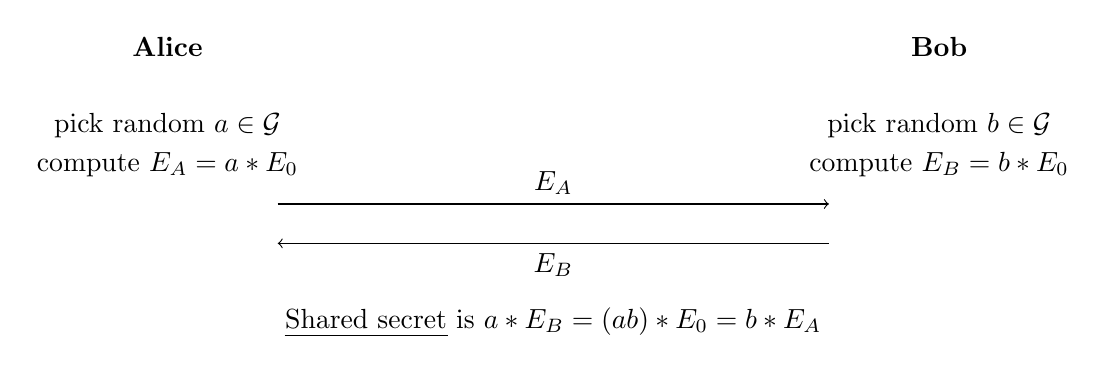
\begin{tikzpicture}[x=1.4cm]
      \node at (0,0) {\bf Alice};
      \node at (7,0) {\bf Bob};
      \node at (0,-1) {pick random \alert{$\a\in\G$}};
      \node at (0,-1.5) {compute $E_A=\a*E_0$};
      \node at (7,-1) {pick random \alert{$\b\in\G$}};
      \node at (7,-1.5) {compute $E_B=\b*E_0$};
      \draw[->]
      (1,-2) to node[auto] {$E_A$} (6,-2);
      \draw[->] (6,-2.5) to node[auto] {$E_B$} (1,-2.5);
      \node at (3.5,-3.5) {\emph{Shared secret} is \alert{$\a*E_B=(\a\b)*E_0=\b*E_A$}};
    \end{tikzpicture}
  \end{center}
\end{frame}

%%

\begin{frame}{Quantum security}

  \textbf{Fact:} Shor's algorithm \emph{does not apply} to Diffie-Hellman
  protocols from \emph{group actions}.

  \begin{block}{Subexponential attack\hfill\emph{$\exp(\sqrt{\log p\log\log p})$}}
    \begin{itemize}
    \item Reduction to the \emph{hidden shift problem} by evaluating
      the class group action in \emph{quantum
        supersposition} (subexpoential cost);
    \item Well known reduction from the hidden shift to the
      \emph{dihedral (non-abelian) hidden subgroup problem};
    \item Kuperberg's algorithm solves the dHSP with a subexponential
      number of class group evaluations.
    \item Recent work suggests that $2^{64}$-qbit security is achieved
      somewhere in $512 < \log p < 2048$.
    \end{itemize}
  \end{block}
\end{frame}

%%

\begin{frame}{A $\Sigma$-protocol from group actions \small(Stolbunov 2008)}
  \begin{columns}
    \begin{column}{0.55\textwidth}
      Building block of Seasign and CSI-FiSh:

      \medskip
      \begin{itemize}
      \item<1-> A key pair \emph{$(\frak{s}, \frak{s}*E)$};
      \item<2-> Commit to a \emph{random element $\frak{r}*E$};
      \item<3-> Challenge with bit \emph{$b\in\{0,1\}$};
      \item<4-> Respond with \emph{$\frak{c} = \frak{r}/\frak{s}^b$};
      \item<5-> Verify that \emph{$\frak{c}*\frak{s^b}*E = \frak{r}*E$}.
      \end{itemize}

      \begin{block}{Zero-knowledge}<6->
        \centering
        Does not leak if:\\
        \alert{$\frak{c}$ is uniformly distributed} and independent from $\frak{s}$.
      \end{block}

    \end{column}  
    \begin{column}{0.40\textwidth}
      \centering
      \begin{tikzpicture}
        \node (g) at (0,0) {$E$};
        \node (gs) at (3,0) {$E_s$};
        \path[->] (g) edge node[auto]{$\frak{s}$} (gs);
        \uncover<2->{
          \node (gr) at (1.5,-3) {$E_r$};
          \path[->] (g) edge node[auto,swap]{$\frak{r}$} (gr);
        }
        \uncover<4->{
          \path[dashed,->] (gs) edge node[auto]{$\frak{r}/\frak{s}$} (gr);
        }
      \end{tikzpicture}
    \end{column}  
  \end{columns}
\end{frame}

%%

\begin{frame}{How CSIDH fails the axioms}
  \begin{block}{\alt<2->{\sout{Hard Homogeneous Space (HHS)}}{Hard
        Homogeneous Space (HHS)} \uncover<2->{Restricted Effective Group Action (REGA)}}
    \emph{$\G\circlearrowright\E$} such that $\G$ is commutative and:
    \begin{itemize}
    \item \emph{Inverting} the action is \emph{hard}.
    \item \alt<2->{\sout{\emph{Evaluating} $E' = \g*E$ is \emph{easy};}}{\emph{Evaluating} $E' = \g*E$ is \emph{easy};}
    \item<2-> There is a small list of elements
      \emph{$(\g_1, \ldots, \g_n)$} such that evaluating $E' = \g_i*E$
      is easy.
    \end{itemize}
  \end{block}
  
  \begin{uncoverenv}<3->
    Assume that $(\g_1, \ldots, g_n)$ generates $\G$:
    \begin{align*}
      \Z^n &\twoheadrightarrow \G\\
      (a_1,\ldots,a_n)&\mapsto \g_1^{a_1}\cdots g_n^{a_n}
    \end{align*}
    Extend $\G\circlearrowright\E$ to an action
    \emph{$\Z^n\circlearrowright\E$} (not free):
    \[(a_1, \ldots, a_n) * E \quad:=\quad \g_1^{a_1} * \cdots * \g_n^{a_n} * E.\]
  \end{uncoverenv}
\end{frame}

%%

\begin{frame}{Crypto from REGAs}
  \[(a_1, \ldots, a_n) * E \quad:=\quad \g_1^{a_1} * \cdots * \g_n^{a_n} * E.\]

  \begin{itemize}
  \item Evaluation efficient for vectors in $\Z^n$ of \emph{small norm};
  \item Key exchange works unmodified;
  \item<2-> Signature breaks down:
    \begin{columns}
      \begin{column}{0.40\textwidth}
        \begin{itemize}
        \item A key pair \emph{$(\vec{s}, \vec{s}*E)$};
        \item Commit to a \emph{random element $\vec{r}*E$};
        \item Challenge with bit \emph{$b\in\{0,1\}$};
        \item \alert{Respond with $\vec{c} = \vec{r} - b\cdot\vec{s}$};
        \item Verify that \emph{$\vec{c}*(b\cdot\vec{s})*E = \vec{r}*E$}.
        \end{itemize}
        Distribution of \alert{$\vec{r}-\vec{s}$} depends on \alert{$\vec{s}$}.
      \end{column}
      \begin{column}{0.40\textwidth}
        \centering
        \begin{tikzpicture}
          \node (g) at (0,0) {$E$};
          \node (gs) at (3,0) {$E_s$};
          \path[->] (g) edge node[auto]{$\vec{s}$} (gs);
          \node (gr) at (1.5,-3) {$E_r$};
          \path[->] (g) edge node[auto,swap]{$\vec{r}$} (gr);
          \path[dashed,->] (gs) edge node[auto]{$\vec{r} - \vec{s}$} (gr);
        \end{tikzpicture}
      \end{column}
    \end{columns}

    \medskip
    Fix: \emph{rejection sampling}. Very expensive!
  \end{itemize}
\end{frame}

%%

\begin{frame}{How to transform a REGA in an Effective Group Action}
  \begin{align*}
    \Z^n &\twoheadrightarrow \G\\
    (a_1,\ldots,a_n)&\mapsto \g_1^{a_1}\cdots g_n^{a_n}
  \end{align*}
  The kernel is an integral lattice $\Lambda$, and
  \emph{$\G \simeq Z^n/\Lambda$}.

  \begin{enumerate}
  \item Compute the kernel $\Lambda$
    \begin{itemize}
    \item In \emph{subexponential} $L(1/2)$ time for CSIDH, or
    \item In \emph{quantum polynomial time} for any group;
    \end{itemize}
  \item Compute generators of $\Z^n/\Lambda$;
  \item Use lattice reduction to convert elements of $\Z^n/\Lambda$ to
    vectors of \emph{small norm}.
  \end{enumerate}

  \pause
  \begin{block}{Applications \small(Beullens, Kleinjung, Vercauteren 2019; D., Meyer 2020)}
    \begin{itemize}
    \item \emph{CSI-FiSh}: reasonably short and not too slow signatures.
    \item If \emph{$\G=\langle\g\rangle$} is cyclic of order
      \emph{$N$}, explicit action \emph{$\Z/N\Z\circlearrowright\E$}:
      $\qquad a * E := \g^a * E$\\
      $\to$ \emph{threshold signatures} via Shamir secret sharing.
    \end{itemize}
  \end{block}
\end{frame}

%%

\begin{frame}{Non-genericity of CSIDH group action}
  \begin{description}
  \item[$\G$] CSIDH-512: \emph{$\Z^{74}$}, CSI-FiSh: \emph{$\Z/N\Z$},\\
    \textcolor{gray}{abstractly: a \emph{class group} of a quadratic imaginary number
    field.}
  \item[$\E$] Supersingular (Montgomery) invariants \emph{$\subset \F_p$}.
  \end{description}

  \medskip
  In CSIDH/CSI-FiSh, There is a \emph{distinguished curve} $E_0$ such that:
  \begin{align*}
    \g^{-1} * E_0 &= -(\g * E_0)\\[1em]
    \textcolor{gray}{(-\vec{a}) * E_0} &\textcolor{gray}{= - (\vec{a} * E_0)}
  \end{align*}
\end{frame}

\begin{frame}{Oblivious Transfer \small(Lai, Galbraith, Delpech de Saint Guilhem 2021)}
  \centering
  \begin{tikzpicture}
    \node at (0,0) {Trusted setup: \emph{$E \ne E_0$}};
    \node at (-4,-1) {Sender: \emph{$m_0, m_1$}};
    \node at (4,-1) {Receiver: \emph{$b\in\{0,1\}$}};
    \node at (4, -2) {$C = (-1)^b(\frak{r} * E)$};
    \node at (-4,-3.5) {$A = \frak{s} * E$};
    \node at (-4,-4.2) {$c_0 = m_0 \oplus H(\frak{s} * C)$};
    \node at (-4,-4.9) {$c_1 = m_1 \oplus H(\frak{s} * (-C))$};
    \node at (4,-6.4) {$m_b = c_b \oplus H(\frak{r} * A)$};
    \draw[->] (2.5,-2.7) to node[auto,swap] {$C$} (-2.5,-2.7);
    \draw[->] (-2.5,-5.7) to node[auto] {$A,c_0,c_1$} (2.5,-5.7);
  \end{tikzpicture}
\end{frame}

%%

\begin{frame}{Hasing to the set}
  Setups require random $E$ such that the \emph{group action relation}
  \[E = \g * E_0\]
  is \emph{unknown} to all parties.

  \bigskip
  Effective Group Action axioms:
  \begin{itemize}
  \item (nearly) uniform random sampling in $\G$;
  \item say nothing on sampling in $\E$.
  \end{itemize}
  For CSIDH, the set $\E$ of supersingular invariants is \emph{sparse}
  in $\F_p$.

  \begin{block}{Open problem}
    Sample random supersingular curves in a way that \emph{does not
      reveal an isogeny chain} to a
    \textit{distinguished}\footnote{Technically, to a curve with small
      degree endomorphisms} curve.
  \end{block}
\end{frame}

%%

\begin{frame}[plain]
  \begin{beamercolorbox}[sep=0.1px,center,wd=\paperwidth,sep=0.5\paperheight]{palette tertiary}
%    \begin{columns}
%      \begin{column}{0.3\textwidth}
%        \includegraphics[height=\paperheight]{labyrinth}
%      \end{column}
%      \begin{column}{0.7\textwidth}
        \Huge\centering Time-delay protocols
%      \end{column}
%    \end{columns}
  \end{beamercolorbox}
\end{frame}

%%

\begin{frame}{Weil pairing and isogenies}
  \centering
  \begin{tikzpicture}
    \node (E) at (0,0) {$E$};
    \node (E1) at (4,0) {$E'$};
    \node at (-1,-1) {$P \to \mathbb{G}_1\times\mathbb{G}_2$};
    \node at (5,-1) {$\mathbb{H}_1\times\mathbb{H}_2 \gets Q$};

    \draw [->] (E) edge[bend left,auto] node {$\phi$} (E1)
    (E1) edge[bend left,auto] node {$\hat\phi$} (E);
  \end{tikzpicture}
  
  \begin{block}{Theorem}
    Let \emph{$ϕ:E→E'$} be an isogeny, let \emph{$e_N$} be the Weil
    pairing of $E$ and \emph{$e_N'$} that of $E'$.\\
    The dual isogeny \emph{$\hat{ϕ}:E'→E$} is the unique isogeny such that
    \[e_N(P,\hat{ϕ}(Q)) = e_N'(ϕ(P),Q),\]
    for any integer $N$ and any points $P,Q$ of order $N$.

    \bigskip
    \textbf{Corollary:} \hfill$e_N'(ϕ(P),ϕ(Q)) = e_N(P,Q)^{\deg ϕ}$.\hfill\strut
  \end{block}
\end{frame}

%%

\begin{frame}{Boneh--Lynn--Shacham (BLS) signatures}
  \begin{block}{}
    \begin{description}
    \item[Private key:] $s∈ℤ/Nℤ$.
    \item[Public key:] $g^s$.
    \item[Sign:] $m ↦ H(m)^s$.
    \item[Verifiy:] $e_N(g,H(m)^s) = e_N(g^s,H(m))$.
    \end{description}
  \end{block}

  \begin{center}
    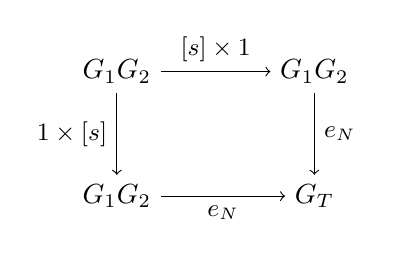
\begin{tikzpicture}[ampersand replacement=\&]
      \matrix(m)[matrix of math nodes,row sep=3em,column sep=4em]{
        \mathbb{G}_1 × \mathbb{G}_2 \& \mathbb{G}_1 × \mathbb{G}_2\\
        \mathbb{G}_1 × \mathbb{G}_2 \& \mathbb{G}_T\\
      };
      \draw[->]
      (m-1-1) edge node[above]{\small$[s]\times 1$} (m-1-2)
      (m-1-1) edge node[left]{\small$1\times [s]$} (m-2-1)
      (m-1-2) edge node[right]{\small$e_N$} (m-2-2)
      (m-2-1) edge node[below]{\small$e_N$} (m-2-2);
    \end{tikzpicture}
  \end{center}
  
  Proof of knowledge of \emph{endomorphism} $x\mapsto x^s$.
\end{frame}

%%

\begin{frame}{US patent 8,250,367 (Broker, Charles and Lauter 2012)}
  \begin{block}{Signatures from isogenies + pairings}
    \begin{description}
    \item[Private key:] an isogeny $\phi$.
    \item[Public key:] $\phi(P)$.
    \item[Sign:] $m ↦ \hat\phi(H(m))$.
    \item[Verifiy:] $e_N(P, \hat\phi(H(m))) = e_N'(\phi(P), H(m))$.
    \end{description}
  \end{block}

  \begin{center}
    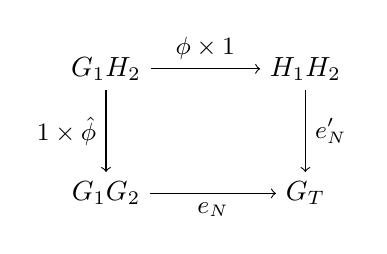
\begin{tikzpicture}[ampersand replacement=\&]
      \matrix(m)[matrix of math nodes,row sep=3em,column sep=4em]{
        \mathbb{G}_1 × \mathbb{H}_2 \& \mathbb{H}_1 × \mathbb{H}_2\\
        \mathbb{G}_1 × \mathbb{G}_2 \& \mathbb{G}_T\\
      };
      \draw[->]
      (m-1-1) edge node[above]{\small$\phi\times 1$} (m-1-2)
      (m-1-1) edge node[left]{\small$1\times\hat\phi$} (m-2-1)
      (m-1-2) edge node[right]{\small$e_N'$} (m-2-2)
      (m-2-1) edge node[below]{\small$e_N$} (m-2-2);
    \end{tikzpicture}
  \end{center}
  
  Proof of knowledge/evaluation of \emph{isogeny} $\phi$.  
\end{frame}

%%

\begin{frame}
  \begin{block}{Verifiable Delay Functions \small(D., Masson, Petit, Sanso 2019)}
    \begin{itemize}
    \item $\phi$ is a \emph{long chain of small degree isogenies} (e.g., degree $2$);
    \item Conjecturally \emph{sequential task}: evaluate one isogeny at a time;
    \item \emph{Fast verification} of evaluation through pairing.
    \end{itemize}
  \end{block}
  
  \begin{block}{Delay Encryption \small(Burdges, D. 2021)}
    \begin{itemize}
    \item Start from \emph{Boneh-Franklin IBE}, replace scalar with isogeny;
    \item Everyone can \emph{encrypt efficiently} to an identity;
    \item \emph{Slow decryption}: need to evaluate long chain of isogenies.
    \end{itemize}
  \end{block}

  \begin{block}{Efficient distributed generation of random supersingular curves}
    \begin{itemize}
    \item Participant $i$ \emph{walks from $E_i$ to $E_{i-1}$} using a
      random chain of isogenies;
    \item \emph{Proves knowledge} of $E_i\to E_{i-1}$;
    \item In the end, \emph{no one knows $E_0 \to E_n$} as long as at
      least one participant is honest.
    \end{itemize}
  \end{block}
\end{frame}

%% 

\begin{frame}[plain]
  \begin{beamercolorbox}[sep=0.1px,center,wd=\paperwidth,sep=0.5\paperheight]{palette tertiary}
%    \begin{columns}
%      \begin{column}{0.3\textwidth}
%        \includegraphics[height=\paperheight]{labyrinth}
%      \end{column}
%      \begin{column}{0.7\textwidth}
        \Huge\centering What else is there?
%      \end{column}
%    \end{columns}
  \end{beamercolorbox}
\end{frame}

%%

\begin{frame}{SIDH and SQISign}
  \small
  \begin{columns}
    \begin{column}{0.5\textwidth}
      \centering
      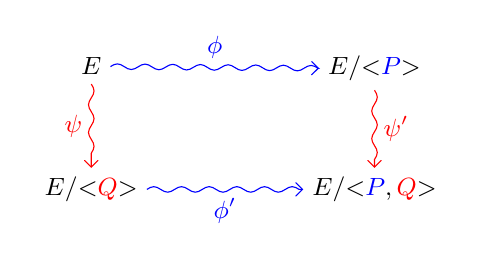
\begin{tikzpicture}[coils/.style={-angle 90,decorate,decoration={coil,aspect=0,amplitude=1pt}}]
        \small
        \node[matrix of nodes, ampersand replacement=\&, column sep=2cm, row sep=1cm] (diagram) {
          |(E)| $E$ \& |(Es)| $E/〈\bl{P}〉$ \\
          |(Ep)| {$E/〈\rd{Q}〉$} \& |(Eps)| {$E/〈\bl{P},\rd{Q}〉$}\\
        };
        \path[->,blue] (E) edge[coils] node[auto] {$\phi$} (Es);
        \path[->,blue] (Ep) edge[coils] node[auto,swap] {$\phi'$} (Eps);
        \path[->,red] (E) edge[coils] node[auto,swap] {$\psi$} (Ep);
        \path[->,red] (Es) edge[coils] node[auto] {$\psi'$} (Eps);
      \end{tikzpicture}

      \begin{itemize}
      \item Secret key spaces: \emph{$\mathbb{K}_2 = \mathbb{P}^2(\Z/2^a\Z)$} and
        \emph{$\mathbb{K}_3 = \mathbb{P}^2(\Z/2^b\Z)$};
      \item Generalizable to more spaces
        $\mathbb{K}_2, \mathbb{K}_3, \mathbb{K}_5, \ldots$
      \item Many traps and pitfalls:
        \begin{itemize}
        \item Active attack\\
          {\footnotesize(Galbraith, Petit, Shani, Ti 2016)}
        \item Too many keyspaces weaken security\\
          {\footnotesize(de Quehen, Kutas, Leonardi, Martindale, Panny,
          Petit, Stange 2021)}
        \end{itemize}
      \end{itemize}
    \end{column}
    \begin{column}{0.5\textwidth}
      \centering
      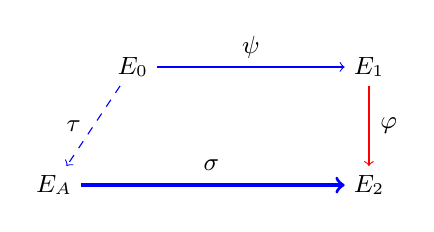
\begin{tikzpicture}
        \small
        \node (E0) at (1,2.5) {$E_0$};
        \node (E1) at (4,2.5) {$E_1$};
        \node (E2) at (4,1) {$E_2$};
        \node (EA) at (0,1) {$E_A$};
        \node (A) at (0.25,1.75) {$\tau$};
        \node (B) at (2.5,2.75) {$\psi$};
        \node (A) at (4.25,1.75) {$\varphi$};
        \node (B) at (2,1.25) {$\sigma$};
        % \draw [->] (E) -- (E1);
        \draw [blue,very thick] [->] (EA) -- (E2);
        \draw [red] [->] (E1) to (E2);
        \draw [blue,dashed] [->] (E0) to (EA);
        \draw [blue] [->] (E0) to (E1);
      \end{tikzpicture}

      \begin{itemize}
      \item A \emph{trapdoor} $\tau$: knowledge of endomorphism ring;
      \item Gives power to construct \emph{``alternate isogeny
          paths''};
      \item NIZK proof of knowledge of endomorphism ring, under
        \emph{new and complicated assumptions};
      \item Lots of parameters to play with.
      \end{itemize}
    \end{column}
  \end{columns}
\end{frame}

%%

\begin{frame}{Summary}
  \begin{itemize}
  \item \emph{Cryptographic Group Actions} are easy to use and powerful, but
    pay attention to details.
    \begin{itemize}
    \item CSIDH (REGA) easier to instantiate, but more limited;
    \item CSI-FiSh very hard to instantiate, but more powerful.
    \end{itemize}
  \item \emph{Isogenies + Pairings} are under-explored, may give more
    than just time-delay primitives.
  \item \emph{SIDH} may be a white whale, but it is a fundamental tool
    nevertheless.
  \item \emph{Endomorphism rings as trapdoors} is the new
    cool.  High potential, but terribly complicated!
  \end{itemize}
\end{frame}

%%

\begin{frame}[plain]
  \centering
  \begin{tikzpicture}[remember picture,overlay]
    \begin{scope}[xscale=1.7,yshift=-15,opacity=0.8]
      \def\crater{12}
      \def\jumpa{-8}
      \def\jumpb{9}
      \def\diam{5cm}

      \foreach \i in {1,...,\crater} {
        \draw[blue] (360/\crater*\i : \diam) to[bend right] (360/\crater*\i+360/\crater : \diam);
        \draw[red] (360/\crater*\i : \diam) to[bend right] (360/\crater*\i+\jumpa*360/\crater : \diam);
        \draw[green] (360/\crater*\i : \diam) to[bend right=50] (360/\crater*\i+\jumpb*360/\crater : \diam);
      }
    \end{scope}
    
    \draw (0,0.5) node{\Huge\bf Thank you};
    \draw (0,-1.1) node{\large\url{https://defeo.lu/}};
    \draw (0,-1.8) node{\large\includegraphics[height=0.9em]{twitter.png}~\href{https://twitter.com/luca_defeo}{@luca\_defeo}};
  \end{tikzpicture}
\end{frame}

%%

\end{document}


% LocalWords:  Isogeny abelian isogenies hyperelliptic supersingular Frobenius
% LocalWords:  isogenous
